\documentclass[tikz,border=8pt]{standalone}
% Shared look for every TikZ diagram. Load with \input{../../tools/tikz-style.tex}
\usepackage[T1]{fontenc}
\usepackage{lmodern}
\renewcommand{\sfdefault}{lmr}  % diagrams use the same serif as the text
\usetikzlibrary{arrows.meta, positioning, shapes.geometric, calc, fit, backgrounds}
\definecolor{cblue}{HTML}{4C78A8}
\definecolor{corange}{HTML}{F58518}
\definecolor{cgreen}{HTML}{54A24B}
\definecolor{cred}{HTML}{E45756}
\definecolor{cpurple}{HTML}{B279A2}
\definecolor{cgrey}{HTML}{6B6B6B}
\tikzset{
  every picture/.style={font=\sffamily, line width=1.2pt},
  box/.style={draw=#1, fill=#1!12, rounded corners=4pt, align=center, inner sep=7pt, minimum height=1.1cm},
  box/.default=cgrey,
  arrow/.style={-{Stealth[length=3mm]}, draw=cgrey, line width=1.4pt},
  title/.style={font=\sffamily\bfseries\Large},
  note/.style={font=\sffamily\small, text=cgrey, align=center},
}
\AtBeginDocument{\hyphenpenalty=10000 \exhyphenpenalty=10000}

\begin{document}
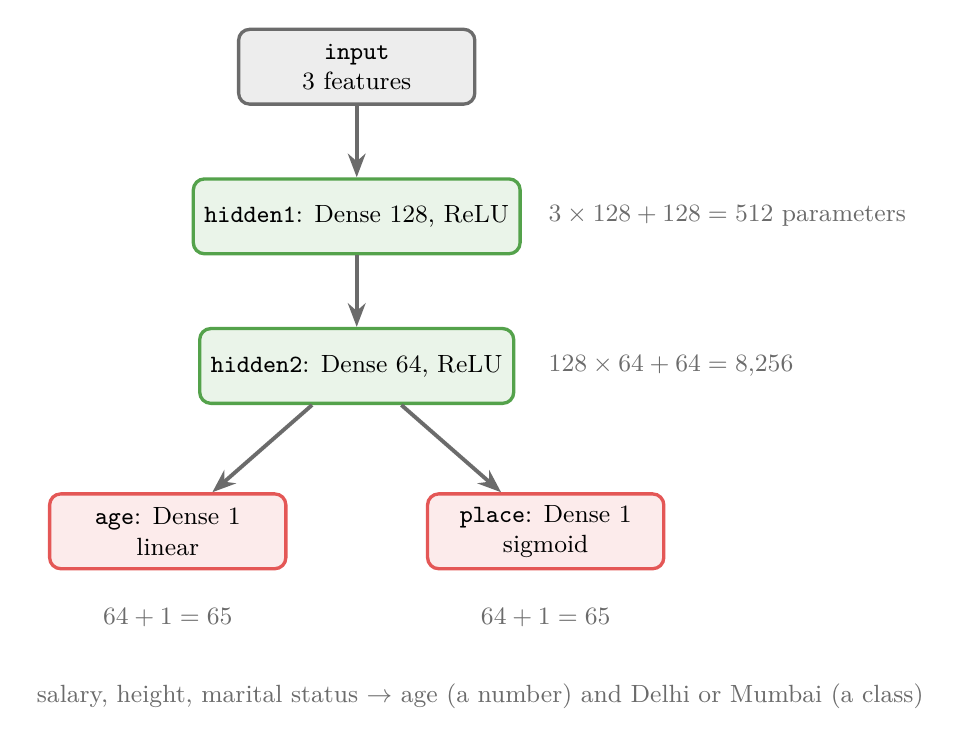
\begin{tikzpicture}[b/.style={box=#1, minimum width=3.0cm, minimum height=0.95cm, inner sep=4pt, font=\sffamily\small},
                    p/.style={note, anchor=west}]
  \node[b=cgrey] (x) at (0, 0) {\texttt{input}\\3 features};
  \node[b=cgreen] (h1) at (0, -1.9) {\texttt{hidden1}: Dense 128, ReLU};
  \node[b=cgreen] (h2) at (0, -3.8) {\texttt{hidden2}: Dense 64, ReLU};
  \node[b=cred] (o1) at (-2.4, -5.9) {\texttt{age}: Dense 1\\linear};
  \node[b=cred] (o2) at (2.4, -5.9) {\texttt{place}: Dense 1\\sigmoid};
  \draw[arrow] (x) -- (h1); \draw[arrow] (h1) -- (h2); \draw[arrow] (h2) -- (o1); \draw[arrow] (h2) -- (o2);
  \node[p] at (2.3, -1.9) {$3 \times 128 + 128 = 512$ parameters};
  \node[p] at (2.3, -3.8) {$128 \times 64 + 64 = 8{,}256$};
  \node[note] at (-2.4, -7.0) {$64 + 1 = 65$};
  \node[note] at (2.4, -7.0) {$64 + 1 = 65$};
  \node[note, anchor=west] at (-4.2, -8.0) {salary, height, marital status $\rightarrow$ age (a number) and Delhi or Mumbai (a class)};
\end{tikzpicture}
\end{document}
